% uklad dokumentu
	\documentclass{article}
	\usepackage{xparse}
	\usepackage[margin=1cm]{geometry}
    \usepackage{enumerate} 
	\frenchspacing
    \linespread{1.2}
    \setlength{\parindent}{0pt}

% jezyk polski
	\usepackage[polish]{babel}
	\usepackage[utf8]{inputenc}
	\usepackage{polski}
 
% pakiety matematyczne
    \let\lll\undefined
	\usepackage{amssymb}
    \usepackage{amsthm}
	\usepackage{amsmath}
	\usepackage{amsfonts}
	\usepackage{tikz}

% hiperlacza
	\usepackage{hyperref}
	\hypersetup{
		colorlinks,
		citecolor=black,
		filecolor=black,
		linkcolor=black,
		urlcolor=black
	}

% wstawianie zdjec
	\usepackage{graphicx} 
	\pagenumbering{gobble}
	

% podstawowe informacje
    \title{Algorytmy i struktury danych - Lista 4}
    \author{P. Cegieła, W. Sęk}

\begin{document} 

\maketitle

\section{Teoretyczna złożoność}
Teoretyczne złożoności algorytmów ($n=|V|$):
\begin{itemize}
\item $k$-random - $k$ losowań ze złożonością $O(1)$ i liczenie wartości ścieżki z $O(n)$, czyli $O(kn)$,
\item $ext-neighbours$ - $n$-krotne przejście po każdym wierzchołku i przejrzenie $\frac{n(n-1)}{2}$ wierzchołków oraz policzenie wartości ścieżki z $O(n)$ daje $O(n^3)$,
\item $2-opt$ - niech $O(m)$ to złożoność przybliżenia początkowego, $l$ to liczba kroków po której się zatrzymujemy, liczenie kosztu elementu z otoczenia to $O(1)$ (przy początkowym stworzeniu tablicy pomocniczej z $O(n)$), otoczenie ma $O(n^2)$ elementów, więc całościowo $O(m+ln^2)$, gdzie $l$ zależy od przybliżenia początkowego.
\end{itemize}
\newpage
\section{Algorytm k-random}
\subsection{Tabela}
\begin{center}
\begin{tabular}{|c|c|c|c|}
\hline
\multicolumn{4}{|c|}{\textbf{Average PRD}}\\
\hline
\textbf{n} & 10-Random & 100-Random & 1000-Random\\
\hline
100 & 6413.9156401721075 & 6007.918586928952 & 5711.806977951733\\
\hline
200 & 5988.615372379403 & 5727.247304868426 & 5522.69171607988\\
\hline
300 & 5888.036831784668 & 5683.792028830031 & 5528.337270981829\\
\hline
400 & 5802.963142088209 & 5631.843379656301 & 5508.994282851\\
\hline
500 & 5779.552537965469 & 5633.505579085746 & 5517.331574583659\\
\hline
600 & 5724.137341197624 & 5578.206097637371 & 5485.583014224162\\
\hline
700 & 5711.069467439124 & 5571.201094319976 & 5476.566562989776\\
\hline
800 & 5677.560472641102 & 5562.185079759854 & 5470.719995332991\\
\hline
900 & 5673.623396583947 & 5548.007479574144 & 5481.1123195262335\\
\hline
1000 & 5650.144622314967 & 5556.232385763668 & 5459.875331845722\\
\hline
\end{tabular}
\end{center}

\subsection{Wykresy}
\begin{center}
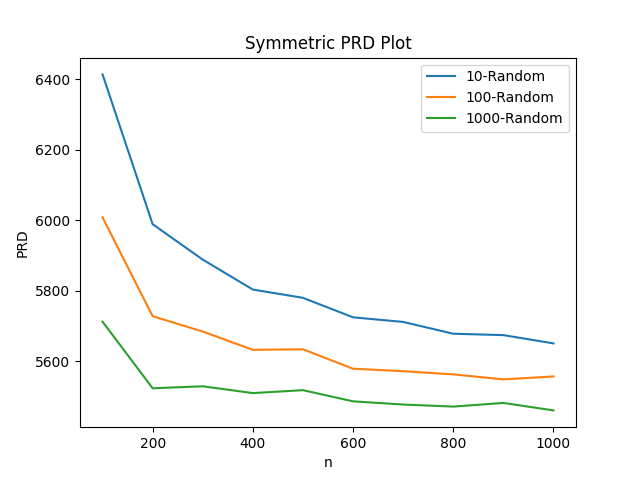
\includegraphics[width=\textwidth, 
                   height = 0.4\textheight, 
                   keepaspectratio]
                  {sym_k_random} 
\end{center}
\begin{center}
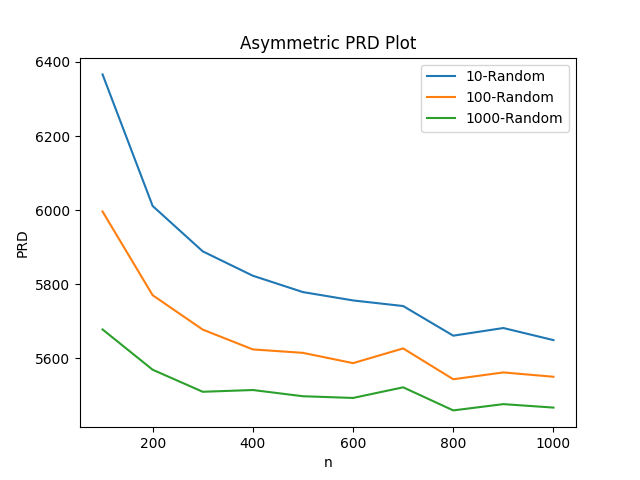
\includegraphics[width=\textwidth, 
                   height = 0.4\textheight, 
                   keepaspectratio]
                  {asym_k_random} 
\end{center}

\begin{center}
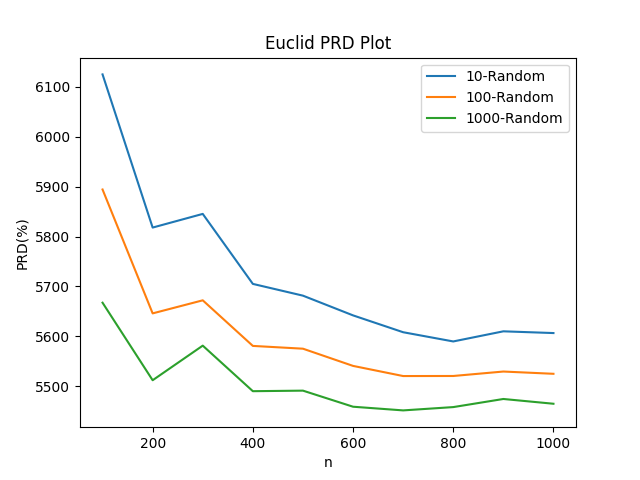
\includegraphics[width=\textwidth, 
                   height = 0.4\textheight, 
                   keepaspectratio]
                  {euc_k_random} 
\end{center}

\subsection{Wnioski}
W każdej rodzinie grafów PRD jest najmniejsze dla $k=1000$ i największe dla $k=10$, ale przy 100-krotnie większym $k$ spadek $PRD$ jest bardzo niewielki. Algorytm $k$-random radzi sobie najlepiej w rodzinie grafów euklidesowych. 

\newpage
\section{Porównanie algorytmów na grafach euklidesowych z TSPLIB}
\subsection{Tabele}
\begin{center}
\begin{tabular}{|c|c|c|c|}
\hline
\multicolumn{4}{|c|}{\textbf{Average PRD}}\\
\hline
\textbf{n} & 1000-Random & Extended-Neighbours & 2-OPT\\
\hline
51 & 306.808 & 103.146 & 91.878\\
\hline
52 & 315.237 & 98.473 & 92.241\\
\hline
70 & 435.881 & 107.926 & 97.704\\
\hline
76 & 444.027 & 111.045 & 94.849\\
\hline
100 & 593.155 & 109.201 & 95.515\\
\hline
105 & 718.542 & 107.776 & 95.285\\
\hline
130 & 656.490 & 105.463 & 93.669\\
\hline
150 & 724.239 & 100.510 & 91.808\\
\hline
225 & 964.538 & 110.576 & 94.255\\
\hline
280 & 1187.883 & 105.355 & 94.110\\
\hline
442 & 1413.942 & 106.094 & 94.210\\
\hline
1002 & 2370.379 & 111.116 & 95.631\\
\hline
\end{tabular}
\end{center}

\begin{center}
\begin{tabular}{|c|c|c|c|}
\hline
\multicolumn{4}{|c|}{\textbf{Average Time}}\\
\hline
\textbf{n} & 1000-Random & Extended-Neighbours & 2-OPT\\
\hline
51 & 31668820 & 4584170 & 8925660\\
\hline
52 & 30858480 & 5042590 & 8846290\\
\hline
70 & 42590610 & 12177150 & 27821070\\
\hline
76 & 47052070 & 15702170 & 34685250\\
\hline
100 & 61385100 & 32708000 & 87529310\\
\hline
105 & 61872570 & 42850460 & 84559130\\
\hline
130 & 74745720 & 67923570 & 131929210\\
\hline
150 & 89032240 & 103249420 & 193264830\\
\hline
225 & 134753750 & 353453680 & 717721220\\
\hline
280 & 166413550 & 664151260 & 1206655960\\
\hline
442 & 271874520 & 2618137660 & 4950646800\\
\hline
1002 & 647387380 & 30213916160 & 72123247190\\
\hline
\end{tabular}
\end{center}

\begin{center}
\begin{tabular}{|c|c|c|c|}
\hline
\multicolumn{4}{|c|}{\textbf{Maximal Time}}\\
\hline
\textbf{n} & 1000-Random & Extended-Neighbours & 2-OPT\\
\hline
51 & 39978600 & 4817900 & 9403300\\
\hline
52 & 31274700 & 5187200 & 9092600\\
\hline
70 & 47594200 & 15057800 & 32388000\\
\hline
76 & 51512200 & 19477600 & 35764400\\
\hline
100 & 65431100 & 34488100 & 96291400\\
\hline
105 & 65726300 & 62679800 & 96151900\\
\hline
130 & 79283500 & 70726100 & 136319200\\
\hline
150 & 91679000 & 105833600 & 197271000\\
\hline
225 & 162636700 & 365920200 & 774637800\\
\hline
280 & 175009000 & 688092700 & 1237435800\\
\hline
442 & 278658100 & 2660588200 & 4975043000\\
\hline
1002 & 806163300 & 30848429200 & 74493868500\\
\hline
\end{tabular}
\end{center}


\subsection{Wykresy}
\begin{center}
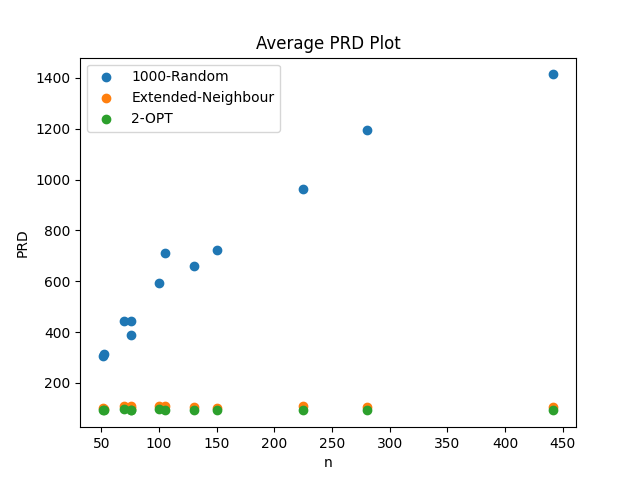
\includegraphics[width=\textwidth, 
                   height = 0.4\textheight, 
                   keepaspectratio]
                  {tsp_lib_prd} 
\end{center}
\begin{center}
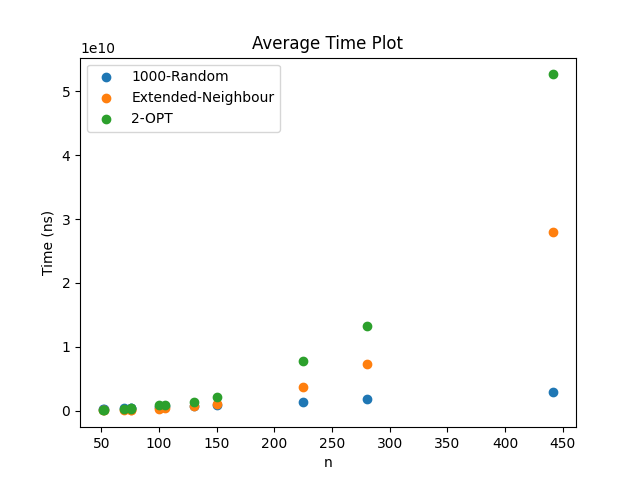
\includegraphics[width=\textwidth, 
                   height = 0.4\textheight, 
                   keepaspectratio]
                  {tsp_lib_avg_time} 
\end{center}

\begin{center}
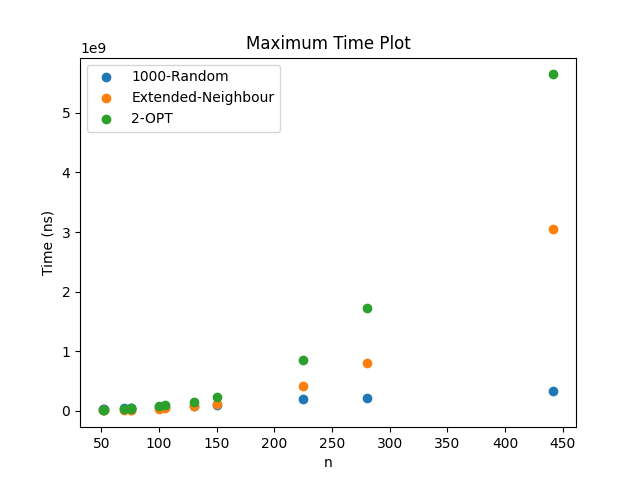
\includegraphics[width=\textwidth, 
                   height = 0.4\textheight, 
                   keepaspectratio]
                  {tsp_lib_max_time} 
\end{center}

\subsection{Wnioski}
W każdej rodzinie grafów PRD jest najmniejsze dla algorytmu $2-OPT$ i największe dla $1000-Random$, natomiast zarówno średnia i jak i maksymalna złożoność czasowa jest największa dla $2-OPT$ i najmniejsza dla $1000-Random$. Złożoność czasowa algorytmu $k$-random jest liniowa, $extended-neighbours$ jest $O(n^3)$, a $2-OPT$ ponad $O(n^3)$, ale niemożliwa do wyznaczenia ze względu na nieznaną liczbę kroków.


\section{Porównanie algorytmów na grafach generowanych losowo}
\subsection{Tabele}

\subsubsection{Grafy asymetryczne}

\begin{center}
\begin{tabular}{|c|c|c|c|c|}
\hline
\multicolumn{5}{|c|}{\textbf{Average Time}}\\
\hline
\textbf{n} & 1000-Random & Neighbours & Extended-Neighbours & 2-OPT\\
\hline
100 & 5215583333 & 28571666 & 2786506666 & 3001888333\\
\hline
200 & 10385900000 & 102848333 & 20872141666 & 21460786666\\
\hline
300 & 15575736666 & 230665000 & 69467785000 & 71687228333\\
\hline
400 & 20725138333 & 400460000 & 161340206666 & 164356600000\\
\hline
500 & 25681436666 & 630796666 & 312382090000 & 319592263333\\
\hline
600 & 31847411666 & 893138333 & 539254811666 & 546289266666\\
\hline
700 & 37347566666 & 1216818333 & 852635371666 & 864857386666\\
\hline
800 & 43085846666 & 1589101666 & 1276754056666 & 1285017576666\\
\hline
900 & 48517803333 & 2017996666 & 1807960408333 & 1825393600000\\
\hline
1000 & 53376455000 & 2458155000 & 2488077001666 & 2527648053333\\
\hline
\end{tabular}
\end{center}

\begin{center}
\begin{tabular}{|c|c|c|c|c|}
\hline
\multicolumn{5}{|c|}{\textbf{Maximum Time}}\\
\hline
\textbf{n} & 1000-Random & Neighbours & Extended-Neighbours & 2-OPT\\
\hline
100 & 53740500 & 296200 & 28250900 & 31605000\\
\hline
200 & 110770900 & 1068300 & 222382100 & 217436400\\
\hline
300 & 156366900 & 2430200 & 699352300 & 730365300\\
\hline
400 & 218396100 & 4173300 & 1630130200 & 1658699700\\
\hline
500 & 272075700 & 6445900 & 3154009300 & 3248476300\\
\hline
600 & 326146900 & 9109900 & 5445648700 & 5518205200\\
\hline
700 & 392337400 & 12303600 & 8644185800 & 8705532900\\
\hline
800 & 442730100 & 16022200 & 12919136400 & 12989845300\\
\hline
900 & 497044800 & 20912700 & 18259475600 & 18320587400\\
\hline
1000 & 545819300 & 25097700 & 25367610900 & 26443099700\\
\hline
\end{tabular}
\end{center}

\begin{center}
\begin{tabular}{|c|c|c|c|c|}
\hline
\multicolumn{5}{|c|}{\textbf{Average PRD}}\\
\hline
\textbf{n} & 1000-Random & Neighbours & Extended-Neighbours & 2-OPT\\
\hline
100 & 144389.48040576265 & 5323.792664503988 & 19.841269841269842 & 0\\
\hline
200 & 264424.58297728904 & 5207.564744303786 & 0 & 0\\
\hline
300 & 344372.7648431962 & 5095.76765521116 & 99.36766034327009 & 0\\
\hline
400 & 454295.2612852427 & 5024.999051480909 & 0 & 0\\
\hline
500 & 542028.8049036451 & 3589.213599432774 & 103.10202617894926 & 0\\
\hline
600 & 699247.4253613068 & 4932.616806843915 & 0 & 0\\
\hline
700 & 755741.8205443585 & 4089.52732594919 & 0 & 0\\
\hline
800 & 808528.5198217536 & 4024.938451458384 & 0 & 0\\
\hline
900 & 926564.7954870298 & 4759.48286220438 & 0 & 0\\
\hline
1000 & 1000638.9406083454 & 3671.7679495233406 & 0 & 0\\
\hline
\end{tabular}
\end{center}


\subsubsection{Grafy symetryczne}

\begin{center}
\begin{tabular}{|c|c|c|c|c|}
\hline
\multicolumn{5}{|c|}{\textbf{Average Time}}\\
\hline
\textbf{n} & 1000-Random & Neighbours & Extended-Neighbours & 2-OPT\\
\hline
100 & 5118872000 & 27634000 & 2761260000 & 4705872000\\
\hline
200 & 10426454000 & 110419000 & 20948980000 & 33434436000\\
\hline
300 & 15504584000 & 235028000 & 69605889000 & 109212242000\\
\hline
400 & 20687462000 & 405624000 & 162160400000 & 246114934000\\
\hline
500 & 25238599000 & 626720000 & 315572915000 & 464210183000\\
\hline
600 & 33565792000 & 908487000 & 552476749000 & 793604803000\\
\hline
700 & 40401877000 & 1304289000 & 891778583000 & 1298559476000\\
\hline
800 & 44722603000 & 1664659000 & 1291840090000 & 1848839045000\\
\hline
900 & 48923905000 & 2028359000 & 1834605650000 & 2642838875000\\
\hline
1000 & 53613716000 & 2543461000 & 2531951057000 & 3497862690000\\
\hline
\end{tabular}
\end{center}


\begin{center}
\begin{tabular}{|c|c|c|c|c|}
\hline
\multicolumn{5}{|c|}{\textbf{Maximum Time}}\\
\hline
100 & 53478300 & 287700 & 28774700 & 59023500\\
\hline
200 & 118932100 & 1496800 & 225860300 & 374150100\\
\hline
300 & 158825400 & 2666500 & 713698900 & 1210248700\\
\hline
400 & 214809200 & 4154100 & 1651365900 & 2783661100\\
\hline
500 & 259651300 & 6437400 & 3196615100 & 4989667500\\
\hline
600 & 369051000 & 9376100 & 5731537000 & 8662696500\\
\hline
700 & 453044000 & 15011700 & 9255213200 & 14112162500\\
\hline
800 & 519034200 & 18486000 & 13176742300 & 20361935900\\
\hline
900 & 542197200 & 21026000 & 18626545300 & 27632920000\\
\hline
1000 & 587381000 & 28130500 & 26359530800 & 38144374100\\
\hline
\end{tabular}
\end{center}

\begin{center}
\begin{tabular}{|c|c|c|c|c|}
\hline
\multicolumn{5}{|c|}{\textbf{Average PRD}}\\
\hline
\textbf{n} & 1000-Random & Neighbours & Extended-Neighbours & 2-OPT\\
\hline
100 & 169641.5152490044 & 8651.420983070748 & 2910.828178233857 & 0\\
\hline
200 & 336491.148021938 & 8695.594682621479 & 3759.5914230406697 & 0\\
\hline
300 & 467506.6707100455 & 9672.03524228703 & 3958.851600018442 & 0\\
\hline
400 & 626451.037540901 & 9242.735074436148 & 4352.368040212525 & 0\\
\hline
500 & 762030.9959416362 & 9491.651021903159 & 3688.834144036091 & 0\\
\hline
600 & 907750.4576801556 & 10564.279122298864 & 3896.5508009869172 & 0\\
\hline
700 & 999294.050859801 & 10511.632970306257 & 4405.698984443974 & 0\\
\hline
800 & 1177366.205236822 & 10932.69827564215 & 4323.395735797874 & 0\\
\hline
900 & 1312890.7423081866 & 9844.799687300712 & 4385.352415182208 & 0\\
\hline
1000 & 1445342.3876189813 & 9645.3501317382 & 4554.947937370816 & 0\\
\hline
\end{tabular}
\end{center}


\subsubsection{Grafy euklidesowe}

\begin{center}
\begin{tabular}{|c|c|c|c|c|}
\hline
\multicolumn{5}{|c|}{\textbf{Average Time}}\\
\hline
\textbf{n} & 1000-Random & Neighbours & Extended-Neighbours & 2-OPT\\
\hline
100 & 5430231666 & 29933333 & 2909718333 & 5610398333\\
\hline
200 & 11033958333 & 108678333 & 22288358333 & 47841571666\\
\hline
300 & 15708336666 & 238925000 & 71815146666 & 149125501666\\
\hline
400 & 21969775000 & 420680000 & 168567516666 & 340063338333\\
\hline
500 & 26306493333 & 644906666 & 327083776666 & 689031216666\\
\hline
600 & 33492466666 & 941325000 & 568170671666 & 1224798638333\\
\hline
700 & 40003946666 & 1280896666 & 907097273333 & 1902227616666\\
\hline
800 & 46368281666 & 1705881666 & 1352010363333 & 2914841420000\\
\hline
900 & 49810670000 & 2115170000 & 1857726728333 & 3970601576666\\
\hline
1000 & 53497760000 & 2547503333 & 2548862593333 & 5568105215000\\
\hline
\end{tabular}
\end{center}


\begin{center}
\begin{tabular}{|c|c|c|c|c|}
\hline
\multicolumn{5}{|c|}{\textbf{Maximum Time}}\\
\hline
100 & 56904000 & 321200 & 30141400 & 66528500\\
\hline
200 & 113894700 & 1158400 & 234500000 & 519662900\\
\hline
300 & 164992700 & 2442400 & 726804400 & 1549853100\\
\hline
400 & 232275800 & 4327000 & 1701320800 & 3590054900\\
\hline
500 & 286456400 & 6665100 & 3415103000 & 7359945700\\
\hline
600 & 349887600 & 9601400 & 5758347300 & 13165101000\\
\hline
700 & 426304400 & 13348700 & 9258026500 & 20301730000\\
\hline
800 & 485403100 & 18255900 & 13873937600 & 31742944800\\
\hline
900 & 510576800 & 21615300 & 18716893000 & 41209877500\\
\hline
1000 & 555995400 & 26168200 & 25734825600 & 57516775300\\
\hline
\end{tabular}
\end{center}


\begin{center}
\begin{tabular}{|c|c|c|c|c|}
\hline
\multicolumn{5}{|c|}{\textbf{Average PRD}}\\
\hline
\textbf{n} & 1000-Random & Neighbours & Extended-Neighbours & 2-OPT\\
\hline
100 & 45057.17215979038 & 2590.834778478913 & 1152.047375520498 & 0\\
\hline
200 & 75024.50161461842 & 2064.382965833475 & 1126.787169849889 & 0\\
\hline
300 & 95586.47736955529 & 2089.941890785232 & 1319.4679540953857 & 0\\
\hline
400 & 115379.31540464885 & 1936.2643602499013 & 1170.3148715360107 & 0\\
\hline
500 & 129969.40868945165 & 1916.510105455013 & 1432.3355018206873 & 0\\
\hline
600 & 147132.99203529008 & 1877.0634799785885 & 1325.9108020407148 & 0\\
\hline
700 & 158377.07578069592 & 1780.3974674441433 & 1334.865053976823 & 0\\
\hline
800 & 173366.5990915691 & 2018.4858325151736 & 1443.038050374855 & 0\\
\hline
900 & 184435.2199324318 & 1859.5850439135654 & 1345.825159240164 & 0\\
\hline
1000 & 197381.2850131005 & 2066.702637095026 & 1479.7361632179882 & 0\\
\hline
\end{tabular}
\end{center}


\subsection{Wykresy}

\subsubsection{Grafy asymetryczne}

\begin{center}
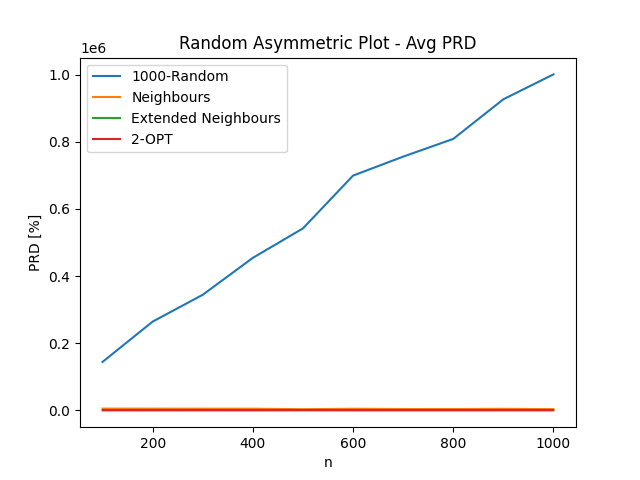
\includegraphics[width=\textwidth, 
                   height = 0.4\textheight, 
                   keepaspectratio]
                  {generated_asym_avg_prd} 
\end{center}

\begin{center}
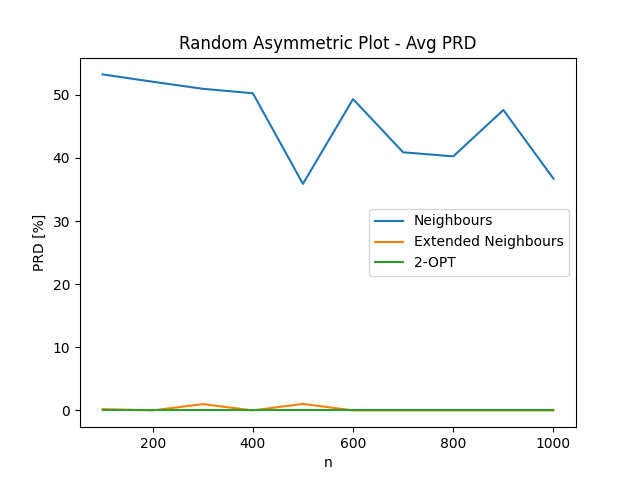
\includegraphics[width=\textwidth, 
                   height = 0.4\textheight, 
                   keepaspectratio]
                  {generated_asym_avg_prd_no_krandom} 
\end{center}

\begin{center}
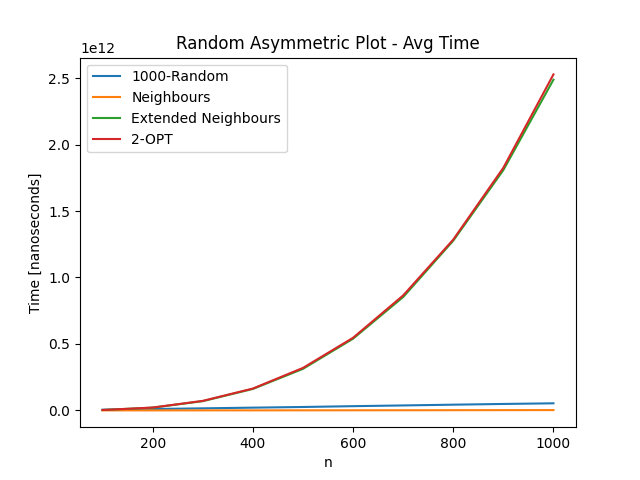
\includegraphics[width=\textwidth, 
                   height = 0.4\textheight, 
                   keepaspectratio]
                  {generated_asym_avg_time} 
\end{center}

\begin{center}
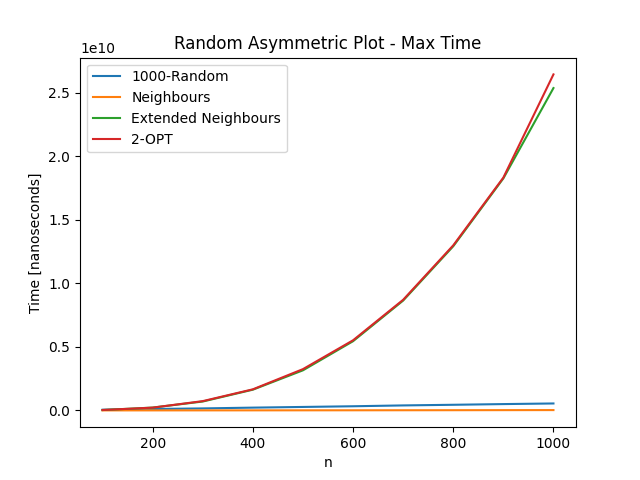
\includegraphics[width=\textwidth, 
                   height = 0.4\textheight, 
                   keepaspectratio]
                  {generated_asym_max_time} 
\end{center}

\subsubsection{Grafy symetryczne}

\begin{center}
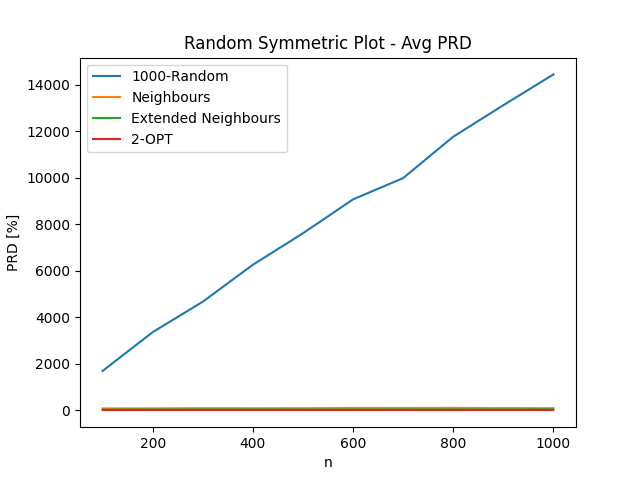
\includegraphics[width=\textwidth, 
                   height = 0.4\textheight, 
                   keepaspectratio]
                  {generated_sym_avg_prd} 
\end{center}

\begin{center}
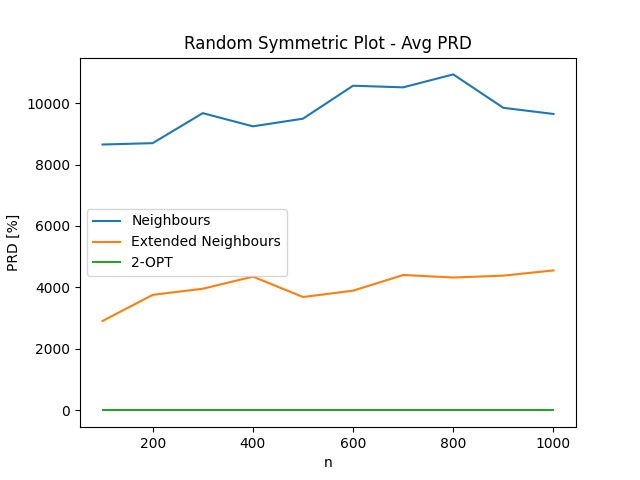
\includegraphics[width=\textwidth, 
                   height = 0.4\textheight, 
                   keepaspectratio]
                  {generated_sym_avg_prd_no_krandom} 
\end{center}

\begin{center}
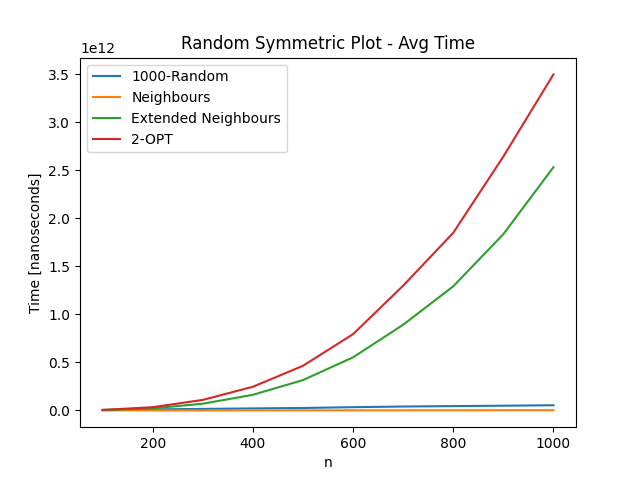
\includegraphics[width=\textwidth, 
                   height = 0.4\textheight, 
                   keepaspectratio]
                  {generated_sym_avg_time} 
\end{center}

\begin{center}
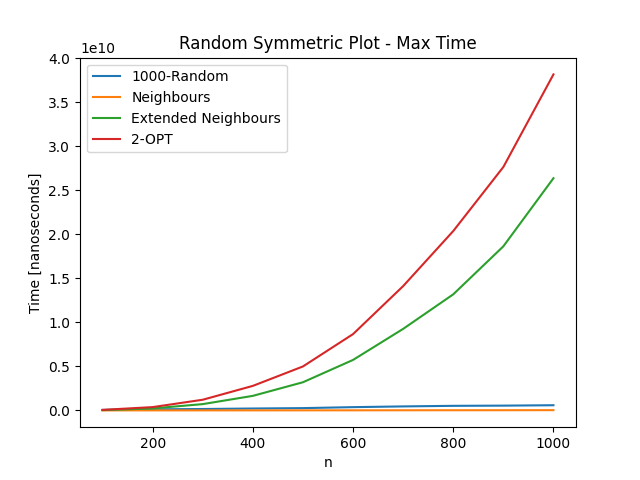
\includegraphics[width=\textwidth, 
                   height = 0.4\textheight, 
                   keepaspectratio]
                  {generated_sym_max_time} 
\end{center}

\subsubsection{Grafy euklidesowe}

\begin{center}
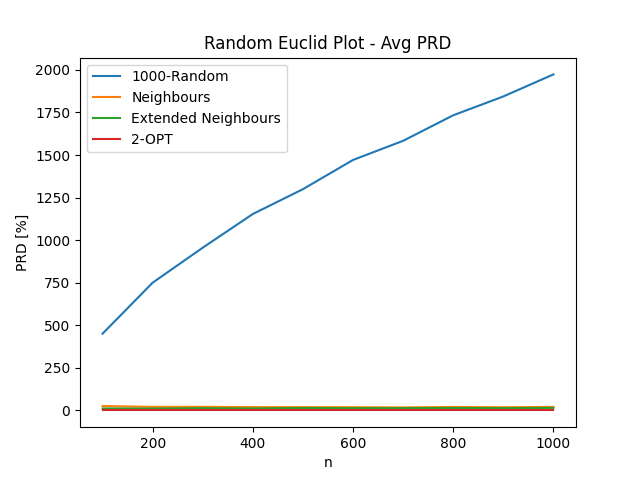
\includegraphics[width=\textwidth, 
                   height = 0.4\textheight, 
                   keepaspectratio]
                  {generated_euclid_avg_prd} 
\end{center}

\begin{center}
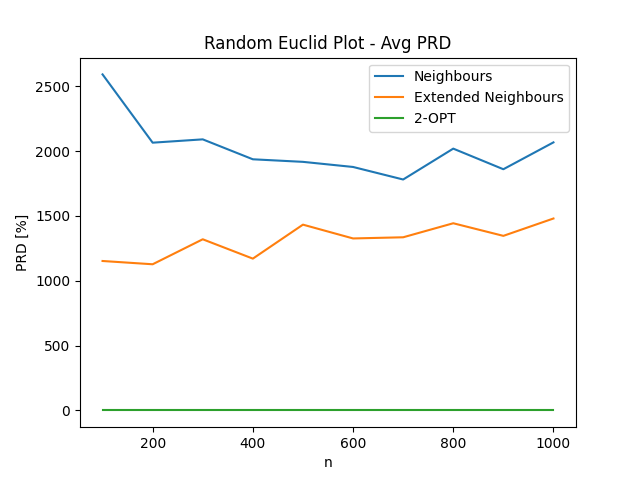
\includegraphics[width=\textwidth, 
                   height = 0.4\textheight, 
                   keepaspectratio]
                  {generated_euclid_avg_prd_no_krandom} 
\end{center}

\begin{center}
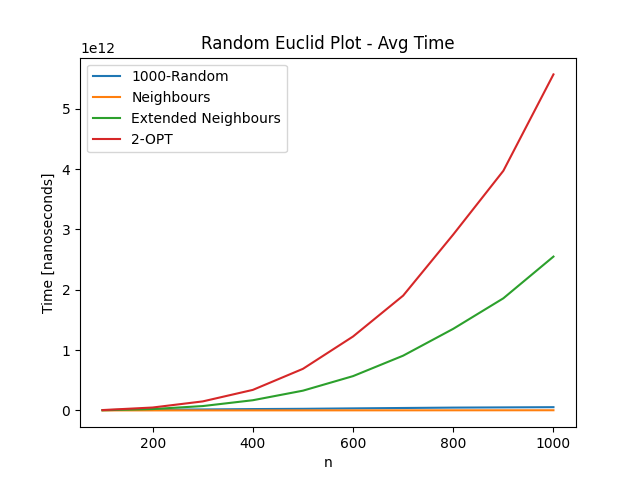
\includegraphics[width=\textwidth, 
                   height = 0.4\textheight, 
                   keepaspectratio]
                  {generated_euclid_avg_time} 
\end{center}

\begin{center}
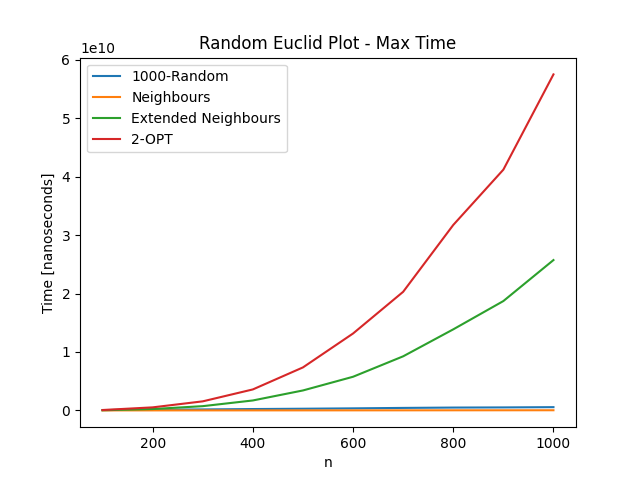
\includegraphics[width=\textwidth, 
                   height = 0.4\textheight, 
                   keepaspectratio]
                  {generated_euclid_max_time} 
\end{center}

\subsection{Wnioski}


\section{Porównanie 2-OPT w zależności od przybliżenia początkowego}
\subsection{Tabele}

\subsubsection{Grafy asymetryczne}

\begin{center}
\begin{tabular}{|c|c|c|c|c|c|c|}
\hline
\multicolumn{7}{|c|}{\textbf{Asymmetric Graphs with 2-OPT}}\\
\hline
 & \multicolumn{2}{|c|}{\textbf{AVG Time}} & \multicolumn{2}{|c|}{\textbf{MAX Time}} & \multicolumn{2}{|c|}{\textbf{AVG PRD}}\\
\hline
\textbf{n} & 1000-Random & Ext-Neighbours & 1000-Random & Ext-Neighbours & 1000-Random & Ext-Neighbours\\
\hline
50 & 48453200 & 6136500 & 3738398333 & 489811666 & 35597.04376268311 & 0\\
\hline
100 & 140853600 & 35301100 & 11970911666 & 3169770000 & 73004.9758129217 & 0\\
\hline
150 & 337295400 & 98910400 & 29113163333 & 9698358333 & 96256.98438783734 & 0\\
\hline
200 & 643440000 & 222620100 & 58731895000 & 21984178333 & 119059.65961691776 & 0\\
\hline
250 & 1392918200 & 438522000 & 123776605000 & 43217630000 & 144661.62881606517 & 0\\
\hline
300 & 1981728700 & 744836600 & 181790746666 & 72750526666 & 168466.84457767615 & 0\\
\hline
350 & 3127470800 & 1156490900 & 294949878333 & 114528933333 & 201839.59192018144 & 0\\
\hline
400 & 4895469300 & 1719545200 & 434607098333 & 170149210000 & 219001.69640333427 & 0\\
\hline
450 & 6997186800 & 2429447700 & 638500593333 & 241024308333 & 231538.9713570598 & 0\\
\hline
500 & 10230351100 & 3378707200 & 905001025000 & 331310758333 & 249834.60481496935 & 0\\
\hline
\end{tabular}
\end{center}


\subsubsection{Grafy symetryczne}

\begin{center}
\begin{tabular}{|c|c|c|c|c|c|c|}
\hline
\multicolumn{7}{|c|}{\textbf{Symmetric Graphs with 2-OPT}}\\
\hline
 & \multicolumn{2}{|c|}{\textbf{AVG Time}} & \multicolumn{2}{|c|}{\textbf{MAX Time}} & \multicolumn{2}{|c|}{\textbf{AVG PRD}}\\
\hline
\textbf{n} & 1000-Random & Ext-Neighbours & 1000-Random & Ext-Neighbours & 1000-Random & Ext-Neighbours\\
\hline
50 & 54974700 & 8059300 & 4912670000 & 742475000 & 435.01603975448376 & 0\\
\hline
100 & 263593200 & 79644600 & 24933430000 & 6215445000 & 296.5871346219297 & 76.26814793409217\\
\hline
150 & 854941600 & 252056300 & 79812985000 & 21103678333 & 562.0643403667292 & 0\\
\hline
200 & 1974940700 & 463551300 & 190022033333 & 43272870000 & 386.77781639316737 & 0\\
\hline
250 & 3901226900 & 977426600 & 381697053333 & 91518833333 & 435.57918990772185 & 0\\
\hline
300 & 6813259300 & 1703896100 & 653903618333 & 152749565000 & 527.1451034832014 & 0\\
\hline
350 & 10818486000 & 2609217900 & 1042695165000 & 247398490000 & 371.06322593105233 & 0\\
\hline
400 & 15996929900 & 4046430100 & 1577727018333 & 354304303333 & 351.7245426245308 & 0\\
\hline
450 & 22753961100 & 5739451900 & 2246563521666 & 524977991666 & 510.1009193872297 & 0\\
\hline
500 & 31306288200 & 7293158000 & 3088863130000 & 682899385000 & 423.6764076969968 & 0\\
\hline
\end{tabular}
\end{center}


\subsubsection{Grafy euklidesowe}

\begin{center}
\begin{tabular}{|c|c|c|c|c|c|c|}
\hline
\multicolumn{7}{|c|}{\textbf{Euclid Graphs with 2-OPT}}\\
\hline
 & \multicolumn{2}{|c|}{\textbf{AVG Time}} & \multicolumn{2}{|c|}{\textbf{MAX Time}} & \multicolumn{2}{|c|}{\textbf{AVG PRD}}\\
\hline
\textbf{n} & 1000-Random & Ext-Neighbours & 1000-Random & Ext-Neighbours & 1000-Random & Ext-Neighbours\\
\hline
50 & 50845700 & 7325400 & 4806420000 & 695278000 & 2596.308721025397 & 0\\
\hline
100 & 236384300 & 50275900 & 22503444000 & 4360152000 & 4683.4335972388535 & 0\\
\hline
150 & 748642900 & 159204100 & 71871182000 & 15081932000 & 4791.206250105386 & 0\\
\hline
200 & 1752181800 & 360983300 & 173144656000 & 33194196000 & 5703.476754080477 & 0\\
\hline
250 & 3597519600 & 719419300 & 336032994000 & 66473034000 & 6640.879179142622 & 0\\
\hline
300 & 6177012400 & 1247142900 & 584690090000 & 115264876000 & 8480.93216294145 & 0\\
\hline
350 & 9811912400 & 2034889600 & 950499916000 & 179479596000 & 8406.706667218925 & 0\\
\hline
400 & 14885090600 & 2743647200 & 1429223796000 & 263122394000 & 9456.626662228227 & 0\\
\hline
450 & 20679005000 & 3990645200 & 2027474658000 & 374963440000 & 10298.344279214956 & 0\\
\hline
500 & 30105890700 & 5752855600 & 2857272732000 & 527189884000 & 10733.905445781715 & 0\\
\hline
\end{tabular}
\end{center}



\subsection{Wykresy}

\subsubsection{Grafy asymetryczne}

\begin{center}
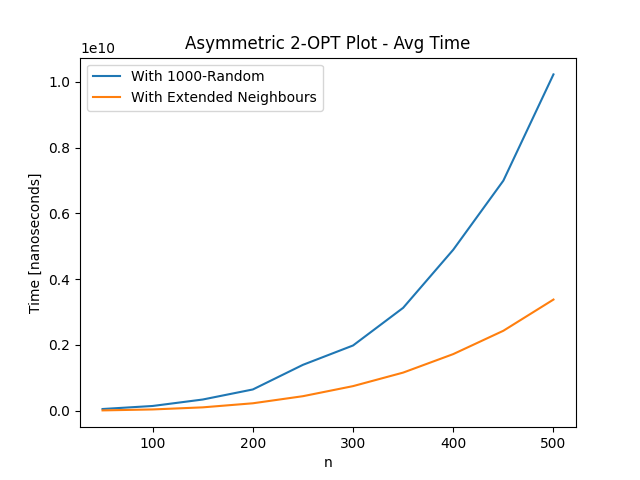
\includegraphics[width=\textwidth, 
                   height = 0.4\textheight, 
                   keepaspectratio]
                  {two_opt_asym_avg_time} 
\end{center}

\begin{center}
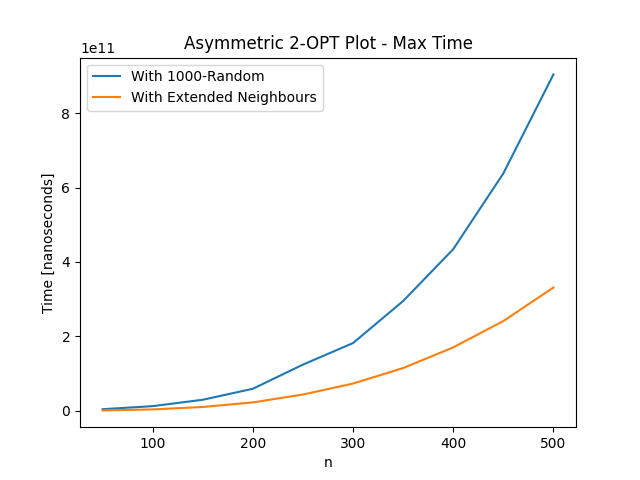
\includegraphics[width=\textwidth, 
                   height = 0.4\textheight, 
                   keepaspectratio]
                  {two_opt_asym_max_time} 
\end{center}

\begin{center}
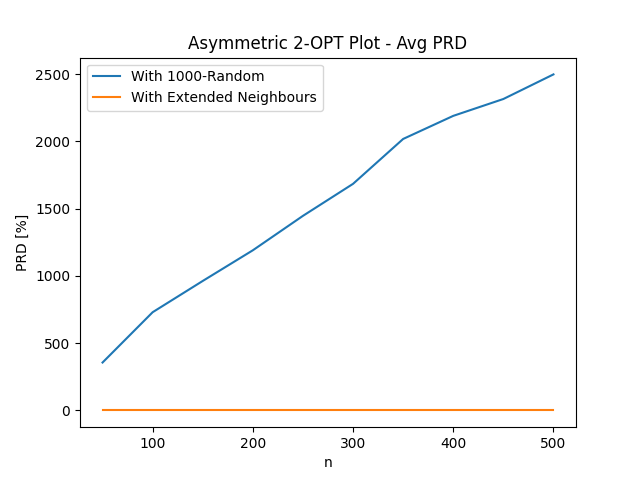
\includegraphics[width=\textwidth, 
                   height = 0.4\textheight, 
                   keepaspectratio]
                  {two_opt_asym_avg_prd} 
\end{center}

\subsubsection{Grafy symetryczne}

\begin{center}
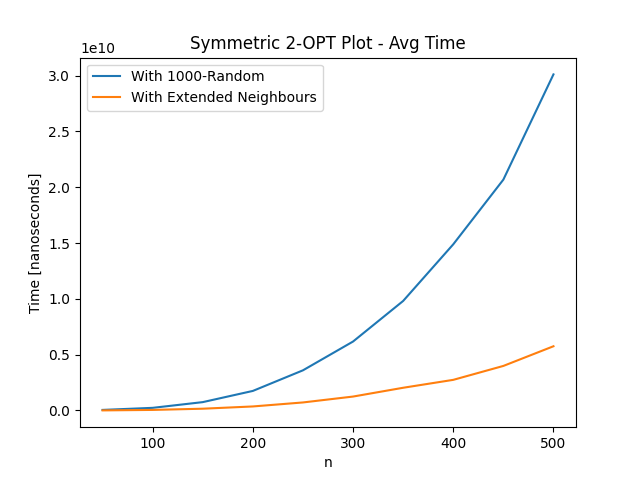
\includegraphics[width=\textwidth, 
                   height = 0.4\textheight, 
                   keepaspectratio]
                  {two_opt_sym_avg_time} 
\end{center}

\begin{center}
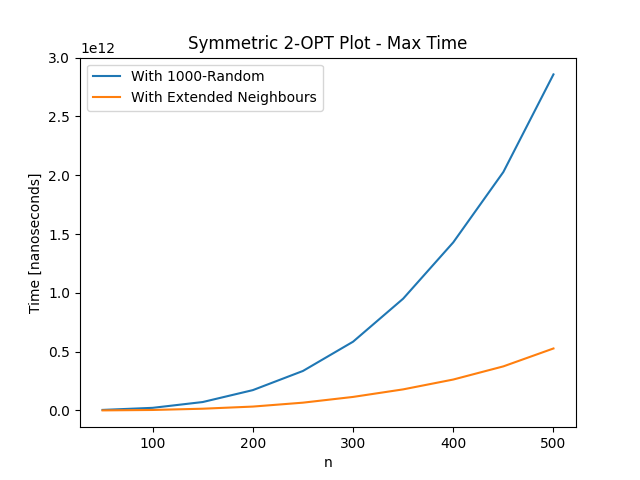
\includegraphics[width=\textwidth, 
                   height = 0.4\textheight, 
                   keepaspectratio]
                  {two_opt_sym_max_time} 
\end{center}

\begin{center}
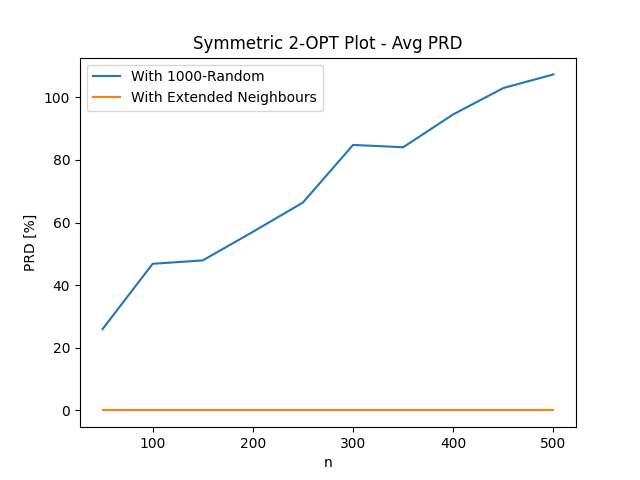
\includegraphics[width=\textwidth, 
                   height = 0.4\textheight, 
                   keepaspectratio]
                  {two_opt_sym_avg_prd} 
\end{center}

\subsubsection{Grafy euklidesowe}

\begin{center}
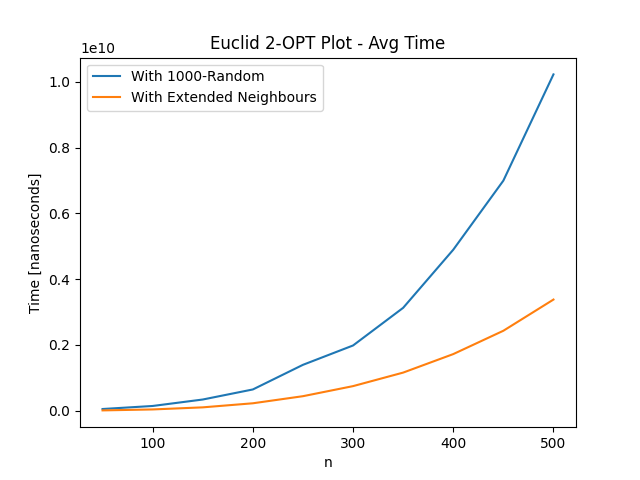
\includegraphics[width=\textwidth, 
                   height = 0.4\textheight, 
                   keepaspectratio]
                  {two_opt_euclid_avg_time} 
\end{center}

\begin{center}
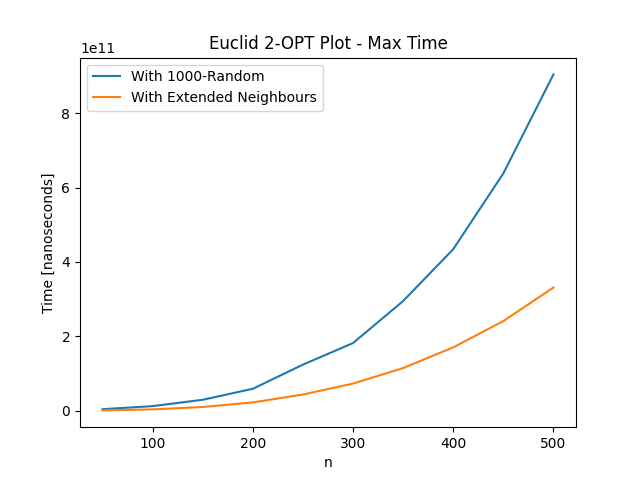
\includegraphics[width=\textwidth, 
                   height = 0.4\textheight, 
                   keepaspectratio]
                  {two_opt_euclid_max_time} 
\end{center}

\begin{center}
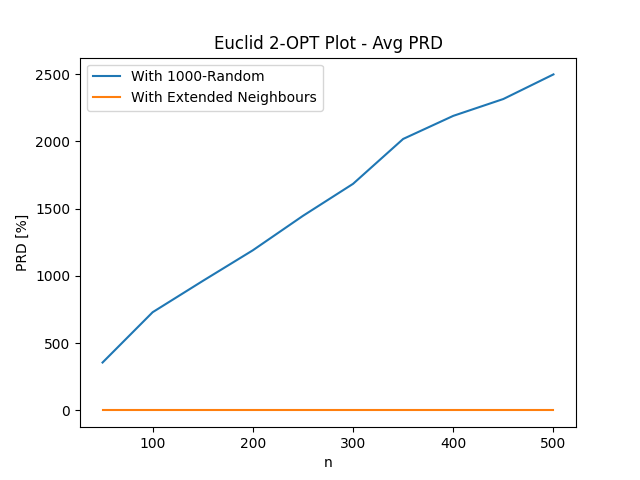
\includegraphics[width=\textwidth, 
                   height = 0.4\textheight, 
                   keepaspectratio]
                  {two_opt_euclid_avg_prd} 
\end{center}
                  
\subsection{Wnioski}

\end{document}